\section{Métodos híbridos}
Esta seção apresenta dois algoritmos de ordenação híbridos, assim chamados por combinarem dois ou mais dos algoritmos discutidos anteriormente.

\subsection{Quicksort com Inserção}
Este algoritmo combina a eficiência do Quicksort para vetores grandes com a do Insercao para vetores pequenos e quase ordenados, como ilustra a Figura \ref{fig:quicksort-insercao}. Ele consiste em duas etapas: a primeira é um Quicksort que ignora subvetores com tamanho menor ou igual a $16$; a segunda é a aplicação do Insercao a todo o vetor. Observe que, ao final da primeira etapa, cada elemento estará, no máximo, a $16$ posições de sua posição correta, de modo que o Insercao executará em tempo linear para finalizar a ordenação.

\begin{figure}[H]
\Caption{\label{fig:quicksort-insercao}Número médio de movimentações realizadas pelos algoritmos Quicksort e Insercao em vetores gerados de forma pseudoaleatória.}
\centering
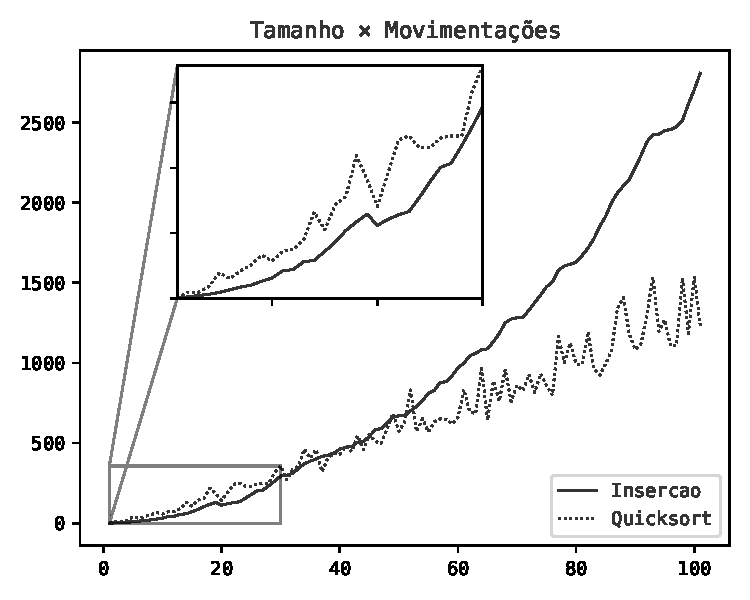
\includegraphics{figuras/pdf/quicksort-insercao.pdf}
\Fonte{Elaborado pelo autor}
\end{figure}

\lstinputlisting[language=C]{codigos/sup/5_quicksort_i.txt}

\subsection{Introsort}
O algoritmo Introsort foi introduzido em \cite{musser1997introspective} e é atualmente utilizado na implementação do método \textit{sort} da biblioteca padrão da linguagem C++.

\subsection*{Outro método de particionamento}
O Introsort controla a altura da pilha de recursão de maneira diferente daquela utilizada no Quicksort, o que possibilita o uso de outro método de particionamento que, como mostra a Figura \ref{fig:particiona_1_2}, realiza menos trocas. Além disso, o elemento pivô é escolhido de forma distinta. A função MoveMedianaFim posiciona, na última posição do vetor, a mediana entre os elementos $v[l]$, $v[(l + r)/2]$ e $v[r]$. Essa estratégia de escolha do pivô é conhecida como ``mediana de três''.
\lstinputlisting[language=C]{codigos/aux/particiona2.txt}

\begin{figure}[H]
\Caption{\label{fig:particiona_1_2}Número médio de trocas realizadas pelos métodos Particiona e Particiona2 em vetores gerados de forma pseudoaleatória.}
\centering
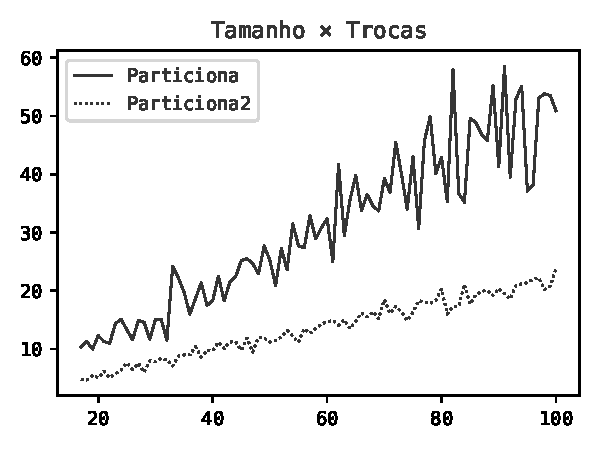
\includegraphics{figuras/pdf/particiona_1_2.pdf}
\Fonte{Elaborado pelo autor}
\end{figure}

\subsection*{O algoritmo Introsort}
A ideia consiste em evitar o pior caso do Quicksort utilizando o Heapsort quando o tamanho da pilha de recursão atinge o valor $\lfloor2\log_2 n\rfloor$. Dessa forma, como o Heapsort possui complexidade no pior caso linearítmica, o pior caso do Introsort é \bigO{n\log_2 n}. Além disso, assim como no algoritmo anterior, o Insercao é utilizado para concluir a ordenação.
\lstinputlisting[language=C]{codigos/sup/6_introsort.txt}
